%---------------------------------------------------------------------------------------------------
% Introduction
%---------------------------------------------------------------------------------------------------
\newpage
%\part{start}
\chapter{Introduction}
	\section{Problem Statement}
		\label{sec:introProblemStatement}
		The main objective that had to be accomplished for the navigation module was, to connect an 
		server/API, which would calculate the appropriate route for the user to reach their end address. 
		This implies that the submodule is responsible for sending queries based upon users 
		current and the end location and in return get a result body which contains
		all the necessary navigation data which would help an visually impaired person to reach their 
		destination.
		
		\par
			The benefit for creating such a system is so that a visually disabled who posses
			the technology can navigate to the desired location without asking for direction
			from a third person. With the help of this module the person would be
			to some extent independent for travelling to unknown places especially. 
	
		\begin{figure}[htbp!]
			\centering 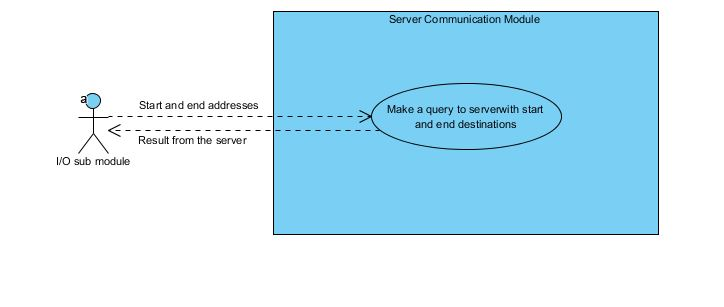
\includegraphics[scale=0.8]{grafiken/googleServerCommunication.jpg}
			\caption{Use case diagram: submodule functionallity}
			\label{fig:Google API communication}
		\end{figure}

	\par
		From the figure \ref{fig:Google API communication} it can be a seen that the API sub-module is 
		just an interface which communicates with the server. It acts as a 
		middleware between the server and the navigation.

	\section{Motivation}
		The major focus of my objectives were related to the software engineering aspects instead of
		the hardware side. I believe that software design is an important part of every project and
		it has always been a challenge to design a project base
		in a way which is robust, scalable and can be maintained with ease. By choosing this package,
		I had the flexibility to develop a system by applying the software design patterns and experiment with 
		the new	technologies available and see them in practice including, what are 
		their advantages and disadvantages. 

	\section{Report Overview}
		Here is a brief outline, providing a short description on what each chapter contains, to get an
		quick overview of the my report.
		
		\paragraph{Chapter 2: "Requirement Analysis"}
			this chapter describes the functional and non-functional objectives of the sub-module. 
		\paragraph{Chapter 3: "Sofware Design"}
			this chapter explains in detail, how the navigation modules software architecture is designed. 
		\paragraph{Chapter 4: "Implementation"} 
			this chapter is where the details of the Implementation decisions and the manual how to understand 
			the project lies.
		\paragraph{Chapter 5: "Testing and Validation"}
			this chapter explains in detail about some test cases which were made to ensure  
			a proper error handling of the module. 
		\paragraph{Chapter 6: "Conclusion"} 
			presents the outcomes and what were the things which could not be completed and some improvements
			which can be done for the future.
